%!TEX root = ../main.tex

\section{Parallelisation}
\label{sec:Parallelisation}

At this point, we aim to develop an efficient parallelization strategy to achieve greater computational efficiency. Initially, we analyzed the bottlenecks in the straightforward implementation of BEM, followed by assessing the performance of the parallelization using both strong and weak scaling analysis.

\subsection{Matrix Assembling and Domain decomposition}
\label{sub:matrix_assembling}

Table~\ref{tb:truncated-py} with computational times refers to the truncated pyramid test case on a single CPU. This test case involves using the BEM to evaluate the solver's performance on a geometrically complex domain shaped like the one in Fig.~\ref{fig:original-6}. It requires handling sharp edges and corners with high accuracy, which poses significant computational challenges.

\begin{table}[hb]
\begin{center}
\caption{Profiling on a single CPU.}\label{tb:truncated-py}
\vspace{-0.5em}
\begin{tabular}{ll}
\hline
Function & Time (s) \\
\hline
Assemble cycle & 68.44 \\
Solvetime & 5.741 \\
Post process (Gradient Recovery) $\qquad$ & 0.1645 \\
Total time & 78.6 \\ 
\hline
\end{tabular}
\end{center}
\end{table}

As we can see, matrix assembly is the major part of the overall program computationally demanding, for this reason, it has to be parallelized. We used a collocation scheme to solve the boundary integral formulation. Provided that the whole computational grid is available on each processor, every line of the matrix can be assembled independently. This is because the process of matrix assembling in BEM involves calculating the interactions
between each basis function and each collocation point across the entire domain. Since each row of the system matrix is basically an integral involving a collocation point and all basis functions, and can be computed independently of others, this matrix assembling task is ideal for parallel execution. For this, we utilized MPI to distribute the task of assembling different rows of the matrix to multiple processors. To preserve the parallelisation efficiency, it is mandatory to achieve a proper work balance between different processors.

\begin{figure}
\begin{center}
    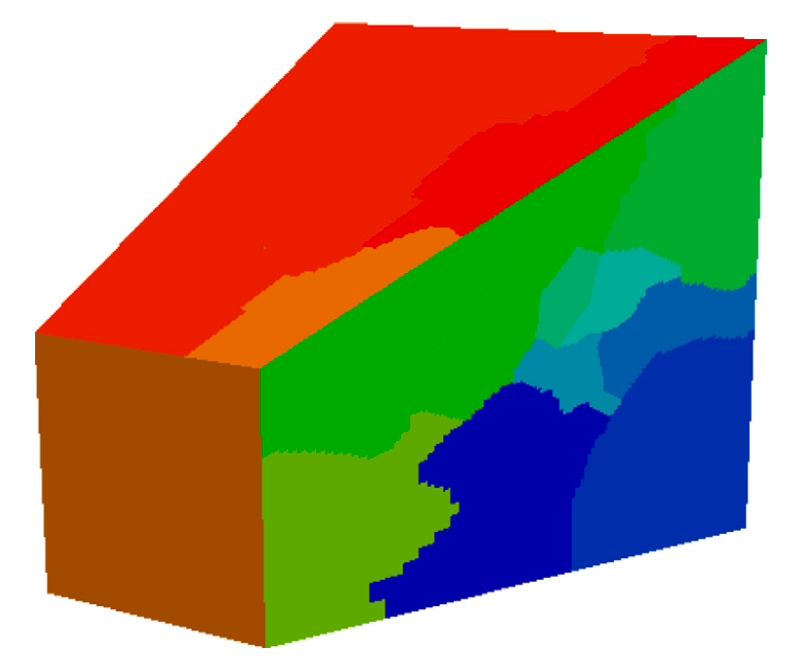
\includegraphics[width=4.2cm]{original-17}    % The printed column width is 8.4 cm.
    \caption{Domain decomposition between 16 different MPI processors.} 
    \label{fig:original-17}
\end{center}
\end{figure}

Fig.~\ref{fig:original-17} indeed represents the domain decomposition between 16 different MPI processors. This non-trivial domain decomposition is due to the local refinement.  It is important to highlight the main difference between BEM and FEM methods, indeed the final matrix in BEM is a smaller but dense matrix, and this is due to the fact that each matrix entry depends on information on the entire boundary of the domain, so every processor still needs access to the full discretisation of the boundary of the geometry, that has not to be confused with the domain decomposition that is related with the
collocation points that every MPI processor has to take into account for a proper workbalance as we mentioned. It could seems that sharing the whole domain to all processor is a bottleneck, but is not, since it is just the boundary domain to be shared, in opposite with the FEM parallelisation method, in which it is mandatory not to share the whole domain. Finally the problem is solved using a parallel implementation of a preconditioned GMRES solver. The preconditioner used is derived from an Incomplete Gauss factorization, which helps reduce the computational load and iteration count necessary for solving.

\subsection{Strong and Weak Scaling}
\label{sub:strong_and_weak_scaling}

The analysis proceeds by evaluating the strong and weak scalability of the previously described problem. We executed a scaling analysis with a total of 40 processors. However, the infiniband network drivers only allow for 16 MPI processors and we will see how this can influence scalability results.

\begin{figure*}
\begin{center}
    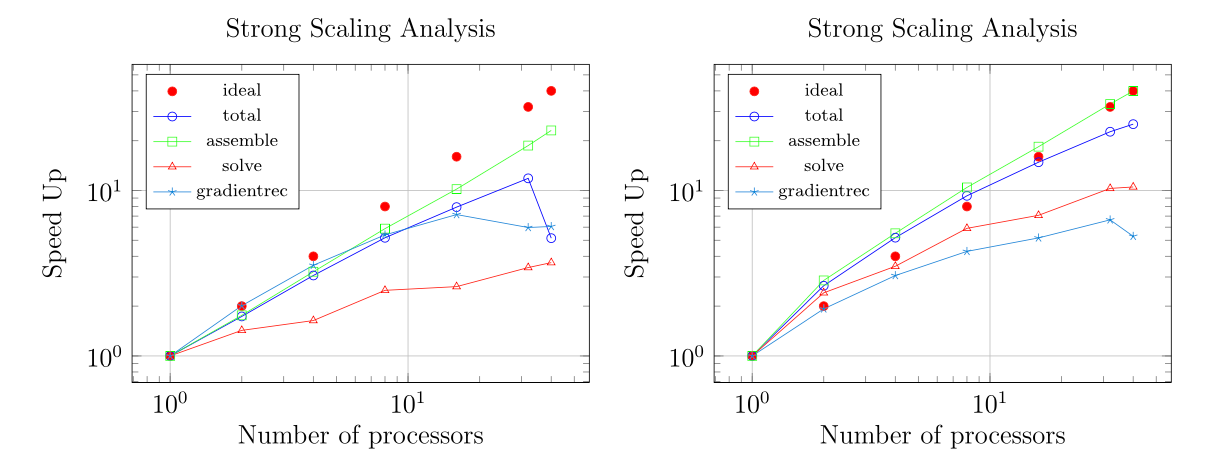
\includegraphics[width=14cm]{original-18}    % The printed column width is 8.4 cm.
    \caption{Strong scalability test. In particular, on the left there is the analysis using 6534 degrees of freedom and on the right the analysis using 25350. In blue with circles we plot the total scalability, in green with squares the performances of the full matrix assembling, in cyan with stars the gradient recovery scalability, and in red with triangles the performance of the linear solver. The red dots represent the ideal speed-up that is of course linear.} 
    \label{fig:original-18}
\end{center}
\end{figure*}

Fig.~\ref{fig:original-18} represents the strong scalability test. As we can see, in the real problem, it is the gradient
recovery and the solve computation that led to a sub-optimal total scalability, and this is even more present in the left graph. This is due to the communication overhead among processors in the
MPI environment because matrix-vector multiplication requires a lot of communication. Notice that the assembly is almost optimal because it doesn’t require any communication. The super optimality in the right test is due to cache resources. We can see an increase in the total performance when considering more degrees of freedom, and this is reasonable because it implies that every MPI processor has to take into account more inner computation,
leading to the communication time becoming less impactful. However, at the same time using more processors involves more communication among them. We could also notice that even
if the solve speed-up is really below the ideal, this doesn’t affect so much the overall performance, and this is due to the relative importance of the assembling versus solving cycles.

Moving forward with the weak scaling, we report the weak scalability analysis in Fig.~\ref{fig:original-20}.

\begin{figure}[htp]
\begin{center}
    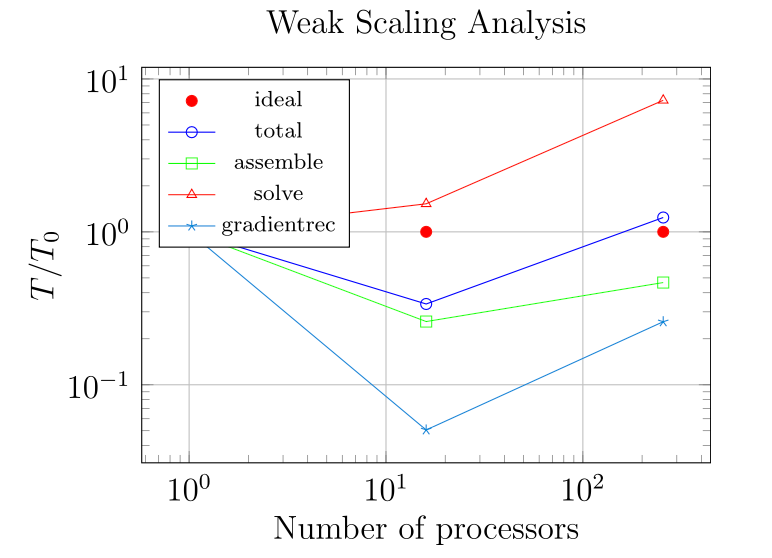
\includegraphics[width=7cm]{original-20}    % The printed column width is 8.4 cm.
    \caption{Weak scalability test. In blue with circles we plot the total performance, in green with squares the timing ratio of the full matrix assembling, in cyan with stars the gradient recovery performance, and in red with triangles the performance of the linear solver. The red dots represents the ideal timings.} 
    \label{fig:original-20}
\end{center}
\end{figure}

The analysis is carried out using up to 256 MPI processors and 25350 degrees of freedom. In particular, we wanted to ensure that each processor handles approximately the same number of matrix entries, thus maintaining a fixed workload per processor in the scaling analysis. If the workload per processor is fixed, we expect that the execution time should remain constant regardless of the number of processors, and the results highlight the desired output. Indeed, the assembling routine has a superoptimal behavior. This is probably due to the structure of the assembling cycle because each processor has to loop over all the cells $N$ times less. However, if we increase the number of MPI processors to 256, we increase dramatically the computational costs for the linear solver, explaining the suboptimal behavior of the solving phase.